\documentclass[letterpaper,10pt,notitlepage]{report}
\usepackage[left=1in,top=1in,right=1in,bottom=1in,nofoot]{geometry}
\usepackage{alltt}
\usepackage{listings}
\usepackage{amsmath}
\usepackage{fancyhdr}
\usepackage{textcomp}
\usepackage{graphicx}
\usepackage{indentfirst}
\usepackage{setspace}
\usepackage[normalem]{ulem}
%\usepackage[bookmarks]{hyperref}
\pagestyle{fancy}

\newenvironment{code}{\begin{quote}\begin{alltt}}{\end{alltt}\end{quote}}
\newcommand{\projname}{\texttt{Cerebro}}

\lhead{\thepage{}}
\rhead{Joseph Colosimo \:\:\: 6.115 \: \projname{}}
\cfoot{}

\setcounter{secnumdepth}{3}
\def\thesection{\arabic{section}}
\def\thesubsection{\arabic{section}.\arabic{subsection}}
\def\thesubsubsection{\arabic{section}.\arabic{subsection}.\arabic{subsubsection}}

\newcommand{\dat}[1]{\texttt{#1}}

\begin{document}

\begin{center}
	\begin{huge}
		\textbf{\projname{} --- A Brainwave Visualizer}
	\end{huge}
\end{center}

\section{Concept}

    \projname{} is a system that uses an EEG to measure electromagnetic
    activity from the surface of the brain and provide a visual display based
    on that activity.  The 8051 microprocessor essentially reads data from an
    EEG device and, though visualization algorithms, computes a display for a
    custom-designed LED panel.

    Hardware communication was done through UART peripheral chips.
    Additionally, the visualization algorithms are customizable through analog
    slider board interface.

    The software was designed to be extremely modular.  The main program calls
    upon libraries to perform tasks such as grabbing and interpreting data
    packets fromt he EEG, reading equalizer slider values, and creating and
    sending packets of data out to the lighting system.

    The attached Appendix A lists all of the code used in development and
    testing.  Roughly 2500 lines out of the total 2911 produced were used in
    \projname{}'s actual final result; the rest constitutes some testing
    applications that proved functionality of the various parts.  I tried to
    comment the code heavily wherever possible to describe in detail my
    motivation for doing various things.  This report covers the way in which
    all the pieces fit together; the code covers the more minute implementation
    details.

\section{Hardware}

    \subsection{Mattel MindFlex with NeuroSky TGAM1}

        In late 2010, a company named NeuroSky began producing low-cost
        low-noise amplifiers designed to read and interpret electromagnetic
        activity at the surface of the brain.  They made this module available
        to a variety of companies.  One such company was Mattel, which used the
        chip in their MindFlex toy whereby the user controls the height of the
        ball by raising or lowering their state of concentration.  Figure
        \ref{fig:mindflex} shows the headband that Mattel created for their toy.

        \begin{figure}[h!]
        \begin{center}
            \includegraphics[scale=.4]{fig/mindflex.png}
            \caption{Hacked MindFlex headband}
            \label{fig:mindflex}
        \end{center}
        \end{figure}

        The internal circuitry in the headband is extremely simple.  NeuroSky's
        TGAM1 EEG daughterboard is soldered onto a mainboard, which has a small
        microcontroller and radio module on it.  The transmission pin from the
        EEG can be sniffed by another microcontroller since the mainboard
        doesn't actually ever need to explicitly control the EEG.

        To prepare the headband, I attached the 5V and ground lines (that would
        normally attached to the battery compartment) to the respective 5V
        supply and ground lines of the Labkit.  I also took the transmission
        line from the EEG chip and wired that out.  To easily control the
        three wires, I used an audio cable to carry the power and signal.
        Given that the EEG draws extremely little current, this was a safe
        design choice.

        The EEG chip outputs data packets at 1-second intervals at 9600 baud.
        An important note is that the NeuroSky chip is configurable in multiple
        ways.  Mattel configures their chip to output data as described, but it
        is also possible to change a jumper such that the EEG outputs raw
        electromagnetic data at 57600
        baud.\footnote{http://wearcam.org/ece516/neurosky\_eeg\_brainwave\_chip\_and\_board\_tgam1.pdf}

        NeuroSky created a two-step packet system.  The outer wrapping of the
        packet syncs a state machine and provides a packet length, payload, and
        checksum.  The inner layer requires a separate state machine to process
        the data and extract the EEG values.  NeuroSky published a document
        describing their packet
        specifications.\footnote{http://weartel.com/ece1766/mindset\_communications\_protocol.pdf}

        In a nutshell, all packets begin with two \dat{SYNC} bytes
        (\dat{0xAA}).  Next, the packet length (\dat{PLEN}) is sent, followed
        by the \emph{payload}, whose length is specified by \dat{PLEN}.
        Finally, a 1-byte, 1's complement checksum value (\dat{CSUM}) is sent
        and the packet is finished.

        Though NeuroSky provides for an enormous amount of capability with
        their packet scheme.  However, the EEG in the MindFlex only provides a
        single set of data and I took advantage of this in my packet processor,
        as I discuss in Section \ref{sec:packetprocessing}.

    \subsection{LED Panel}

        This past January 2011, a small group of my friends and I constructed a
        powerful lighting system designed for adding interesting ambiance to
        events such as parties.  The system had around two dozen instruments of
        three different kinds: 24-bit color panel displays, blacklights/strobe
        light devices, and 24-bit color back-reflected displays.

        As the lead electronics designer of the system, I created a board that
        would take serial input from an RS485 network and feed it to an ATMEGA
        microcontroller.  The serial data would be arranged in packets that
        would control each element of the lighting system.  Communication
        currently runs at 38400 baud.  We have published our protocol and other
        relevant documentation on a
        Wiki.\footnote{http://next-make.mit.edu/wiki/}
        
        The 8051 uses a separate UART peripheral chip to communicate with the
        LED panel as well as a clone of the MAX485 level shifter to create a
        RS-485 compliant waveform that is transmitted via CAT-5 cable.

    \subsection{Equalizer Board}

        A final piece of \projname's hardware is a circuit board containing
        several dozen sliders that was taken from surplus audio equalizer
        equipment.  This board simply has a series of pads on the back of it.
        So, by using an analog de-multiplexer, it's possible to ``scan" through
        the sliders (which are just sliding potentiometers in a voltage divider
        configuration) and read their analog values.  Those values can then be
        used for fine-tuning some values in the visualization algorithms.

        The only defect in the equalizer board was the presence of excess blobs
        of solder, so after quickly resolving that issue, I was able to wire it
        up and get it working.  The sliders are in an odd configuration; every
        other slider seems to be connected to a different piece of circuitry.
        I ended up using a set of sliders that were all connected to two pads.
        These sliders are logarithmic.

        \pagebreak

\section{Hardware Interface Architecture}

    Figure \ref{fig:hwarch} shows the overall architecture of \projname{}.
    Full schematics are located on the next page.

    \begin{figure}[h!]
    \begin{center}
        \includegraphics[scale=.5]{fig/blockdiagram.pdf}
        \caption{Hardware block diagram}
        \label{fig:hwarch}
    \end{center}
    \end{figure}

    \subsection{Reading EEG Data}

        The EEG outputs data at 9600 baud on a TTL-level UART line.  Therefore,
        the 16C450 8051-compatible UART peripheral chip was a natural choice
        for reading data from the device.  The device uses addresses
        \dat{0xFE00} -- \dat{0xFE07} (using a 74LS138 chip selector).  The
        chip's interrupt line is also used (it is passed through an inverter to
        make it compatible with the 8051, which uses an active low interrupt).
        The 16C450 is driven by an 1.8432 MHz clock and has an internal divider
        configuration set to $1.8432e6/16/9600 = 12$ (with no error).  The
        interrupt line is tied to P3.2, which is configured to be an external
        interrupt line.

    \subsection{Reading Equalizer Slider Values}

        \projname{} uses 8 sliders to adjust relative gain data and other
        configurations.  To read data from these sliders, a 5V signal is
        applied across all of them and the 8051 controls (through some free
        lines on its Port 1) a 74HC4067 analog multiplexer/demultiplexer.  The
        Demux is made to ``scan" through the 8 sliders and output the analog
        result to an ADC0804 analog-to-digital converter, which makes available
        for the 8051 a digital value representing the state of the slider.  The
        ADC has address \dat{0xFE10}.

    \subsection{Sending Data to the LED Panel}

        A second 16C450 (running off the same 1.8432MHz clock) is needed to
        output data to the LED panel because the panel requires 38400 baud
        communication.  The divisor configuration for this chip is therefore
        $1.8432e6/16/38400 = 3$ (with no error).  I originally tried using a
        2MHz oscillator to control the device, but the error was too high.
        This chip uses addresses \dat{0xFE20} -- \dat{0xFE27}.  The output of
        the UART is sent to a SN75176B RS-485 level converter, whose output is
        sent to a RJ45 jack.

\section{Software Architecture}

    Figure \ref{fig:swarch} describes \projname{}'s overall software
    architecture.  An external interrupt handler processes incoming data
    packets from the EEG through a state machine, storing the results to a
    series of buffers and alerting the main loop when data is valid.  The main
    loop reads the EEG data, scans the equalizer board sliders, and runs a
    visualization algorithm on the data.  It then starts a timer which
    transitions the old LED output to the new one smoothly.  This transition is
    necessary because the EEG only outputs samples once per second.

        \begin{figure}[h!]
        \begin{center}
            \includegraphics[scale=.4]{fig/software.pdf}
            \caption{Software architecture overview}
            \label{fig:swarch}
        \end{center}
        \end{figure}

    This architecture makes extensive use of defined constants to maximize
    modularity.  Constants prefixed with \dat{Vm\_} represent addresses of
    memory locations where a value will be stored (e.g. \dat{0x70}).  Constants
    prefixed with \dat{Va\_} represent physical hardware addresses (e.g.
    \dat{0xFE03}).  All memory accesses are indirect, so any memory value used
    can be moved into any part of the available internal RAM.  Therefore, the
    \dat{0x80}--\dat{0xFF} realm which requires indirect addressing can be
    used.

    Additionally, for their functions, all libraries use the format
    \dat{F\_XX\_YYY} where \dat{XX} is a 2-character library prefix and
    \dat{YYY} is a function name.  Labels within a library use that function
    format followed by a label description (i.e. \dat{F\_XX\_YYY\_ZZZ}).

    \subsection{EEG Packet Processing}
        \label{sec:packetprocessing}

        \dat{eegctrl.asm} contains an EEG packet processing library.  The
        library contains an initialization routine that sets the 16C450 up for
        8-bit, no-parity, serial communication at 9600 baud.  Furthermore, it
        sets up the chip to deliver an interrupt when it receives data and sets
        up the 8051 to receive this interrupt and run the appropriate packet
        processing handler.

        The packet processor is a combination of a state machine and a payload
        data extractor.  The state machine, as described by Figure \ref{fig:sm}
        reads the outer layer of the EEG packet by waiting for two sync
        signals, getting a packet length, reading a packet into some buffer
        space, and then reading and checking a checksum.  If the checksum
        validates, the payload data extractor is called.

        \begin{figure}[h!]
        \begin{center}
            \includegraphics[scale=.4]{fig/sm.pdf}
            \caption{Packet processor state machine}
            \label{fig:sm}
        \end{center}
        \end{figure}

        The extractor is technically supposed to be a separate state machine
        that reads a data field type and then the associated data for that
        field.  For example, in a typical payload, the first byte will be
        \dat{0x02} to indicate that the byte that follows will be the signal
        quality.  NeuroSky's specification states that the payload does not
        necessarily have to have any specific ordering of data fields.
        However, it seems as though they have built in an impressive amount of
        future-proofing.  After extensive testing, I discovered that the chip
        outputs only one type of payload.  To simplify the library, I decided
        to take advantage of this and always read the same byte offsets of the
        payload into a set of memory addresses.

        If the payload is 32 bytes, then we read and store the data as
        described in Table \ref{tbl:payload}.  The third column of the table
        shows where in 8051 memory the data is stored for the visualizer to
        use.

        \begin{table}[h!]
            \caption{32-Byte payload structure, with important values emphasized}
            \label{tbl:payload}
            \begin{center}
                \begin{tabular}{c|c|c}
                    \hline
                    \hline
                    \textbf{Offset} & \textbf{Description} & \textbf{Storage Address} \\
                    \hline
                    \dat{00} & Signal Quality Command (\dat{0x02}) & --- \\
                    \dat{01} & \textbf{Signal Quality Value} & \dat{Vm\_eeg\_sgnl} \\
                    \dat{02} & FFT Values Command (\dat{0x83}) & --- \\
                    \dat{03} & \# of FFT Values (\dat{0x18}) & --- \\
                    \dat{04}--\dat{27} & \textbf{FFT Values} & 
                        \dat{Vm\_eeg\_dlta}--\dat{Vm\_eeg\_dlta+23} \\
                    \dat{28} & Attention Command (\dat{0x04}) & --- \\
                    \dat{29} & \textbf{Attention Value} &  \dat{Vm\_eeg\_attn} \\
                    \dat{30} & Meditation Command (\dat{0x05}) & --- \\
                    \dat{31} & \textbf{Meditation Value} & \dat{Vm\_eeg\_mdtn} \\
                    \hline
                    \hline
                \end{tabular}
            \end{center}
        \end{table}

    \subsection{Equalizer Board Reader}

        Reading the slider values on the equalizer board is a relatively simple
        task.  \dat{eqboard.asm} contains a library which provides a scan
        function.  This routine sets the demux address to \dat{0}, reads the
        value from the ADC into a memory buffer starting at
        \dat{Vm\_eqb\_vals}, increments the pointer and the demux address, and
        repeats the process 7 more times.  The main loop runs this routine just
        before running the visualization algorithm.

    \subsection{Serial Communication}

        To provide interesting EEG information and aid in debugging,
        \dat{sercom.asm} borrows functions from
        \emph{minmon}\footnote{http://web.mit.edu/6.115/www/miscfiles/minmon.asm}
        that allow the program to initialize a 9600-baud serial communication
        channel and print characters or hex representations of characters.  The
        function \dat{F\_dbg\_prtdata} makes uses of this library to print out
        some data in the format:

        \begin{verbatim}
[signal quality] [attention] [meditation]
 [equalizer values 0-7]
 [eeg fft values 0-23]
        \end{verbatim}

    \subsection{Signal Processor}

        The signal processor fundamentally reads data from the sliders and EEG
        and produces RGB output to the \dat{Vm\_led\_argbuf} buffer.  This
        library is located in \dat{sigproc.asm}.

        If the signal quality is insufficient to produce a reasonable
        visualization, the processor invokes a routine that produces a green
        gradient bar showing the signal quality.  As the quality gets better,
        the bar extends and gets brighter.  If the EEG does not sense any
        signal at all, the signal processor will set all of the pixels to be
        red.

        If the signal quality is sufficient, however, the processor invokes one
        of a few possible algorithms.  I developed numerous algorithms that
        used the EEG data in a variety of ways, and ended up leaving three in
        the code.  The first sets the hue of the first two pixels based on the
        attention value and the hue of the second two based on the meditation
        value.  It sets the brightness of the pixels according to the change in
        the attention and meditation values respectively since the last sample.
        It showed some promise, but I decided to directly used the FFT values
        instead of these composite values.

        I experimented with numerous algorithms and left two of them in the
        code.  The first of these two was an early test.  It simply sets the
        brightness of each pixel based on the value of the theta, low alpha,
        low beta, and mid gamma FFT values.  It doesn't use the equalizer
        sliders or change the hue.

        The second of these two was the final algorithm I came up with.  Though
        it's far simpler than some of the other algorithms I designed and
        eventually scrapped, it seems to be very responsive to change in brain
        activity.  Pixel 0 is set as follows:
        \begin{align}
            P_{0,\textrm{hue}} &= P_{0,\textrm{hue}} \cdot
                (1-\textrm{Slider}_4) + \textrm{NewColor} \cdot \textrm{Slider}_4  \\
            P_{0,\textrm{val}} &= P_{0,\textrm{val}} \cdot
                (1-\textrm{Slider}_5) + \textrm{NewVal} \cdot \textrm{Slider}_4
        \end{align}

        Where \emph{NewColor} is red (\dat{0}) if the scaled delta value is
        higher than the scaled theta value and yellow ($60/360*255=$\dat{42})
        otherwise and \emph{NewVal} is the average of the scaled delta and
        theta values.

        Likewise, pixels 1 through 3 are set similarly using low alpha, high
        alpha; low beta and high beta; and low gamma and mid gamma
        respectively.  The hues each have a 60-degree offset from each other
        (e.g. pixel 3 ranges from cyan to dark blue).
        
    \subsection{Transition System}

        The EEG only provides samples at a rate of once per second, so a method
        of smoothly transitioning one visualization frame to another is
        absolutely necessary.  Normally, a HSV-based transition is preferred
        for color mixing, but for simplicity's sake, I decided to go with a
        simple linear RGB transition because the degree transition between
        samples is usually small enough that it approximates a HSV transition.
        \dat{trans.asm} provides a transition system library.

        The transition system provides an input buffer at
        \dat{Vm\_led\_argbuf}.  The signal processing algorithm always saves
        its result here.  Then, this buffer is copied to one of two other
        buffers.  An interrupt running at 3600Hz (timer value \dat{0x00})
        crossfades from one buffer to another by taking a weighted average of
        the two buffers, saving the result to the \dat{Vm\_led\_rgbargs}
        buffer and calling the LED panel library's function to set the panel's
        pixels.  By continuously swapping the buffer that
        \dat{Vm\_led\_argbuf} gets copied to, the transition system can
        continuously and smoothly transition between successive samples.

        \dat{Vm\_led\_argbuf} is actually technically not necessary because
        one could just pass a pointer to the signal processor to one of two
        buffers.  However, adding this extra buffer provides a better boundary
        that abstracts away the intricacies of the transition system from the
        signal processor.  There's plenty of memory to have an extra buffer.

    \subsection{LED Panel Output}

        Sending data to the LED panel is handled by the library located in
        \dat{ledpanl.asm}.  An initialization function sets up the 16C450 for
        38400 baud, 8-bit, even-parity communication.  \dat{F\_lp\_sendbyte} is
        an auxiliary function that sends a single byte over the 16C450.  A
        function that sets the whole panel was created for debugging purposes
        but is no longer used.  All functionality for output is now used in a
        function that sets each pixel from a buffer located at
        \dat{Vm\_led\_rgbargs}.  The format of the buffer is
        \dat{[RED0][GRN0][BLU0][RED1][GRN1][BLU1][RED2][GRN2][BLU2][RED3][GRN3][BLU3]}.

    \subsection{Color Utilities}

        \dat{colutils.asm} contains a library for processing color.  Currently
        it only has a utility to convert colors in HSV space to RGB.  This
        utility is useful because the signal processing algorithm processes
        values in HSV space, but the LED panel requires RGB inputs.  The
        \dat{hsv2rgb} function performs this task.  The comments in this file
        fully explain the calculation fully.  They were modeled after an
        algorithm described on
        Wikipedia.\footnote{http://en.wikipedia.org/wiki/HSL\_and\_HSV}

\section{Results}

    Determining an appropriate signal processing algorithm was the most
    difficult aspect of this project.  The EEG provides a wealth of data, but
    it is largely useless without an algorithm that shows deep understanding of
    the data.

    The final algorithm I developed comes close to what I wanted, but there's
    always room for improvement.  Furthermore, EEGs with multiple sensors
    provide much more accurate data than EEGs with a single sensor.  They can
    also distinguish between different patterns of thought better based on
    which parts of the brain show the most activity.

    The equalizer board provides a nice way of performing fine-tuned
    adjustments to the output.  The sliders do the following:

    \begin{table}[h!]
        \caption{Equalizer board functionality}
        \begin{center}
            \begin{tabular}{c|c}
                \hline
                \hline
                \textbf{Slider} & \textbf{Function} \\
                \hline
                1 & Master Gain Control \\
                2 & Transition Speed \\
                3 & Algorithm Selector (algorithms 1--3, \\
                  & and then the signal quality meter) \\
                4 & Hue EWMA Ratio \\
                5 & Pixel 0 Value EWMA Ratio \\
                6 & Pixel 1 " \\
                7 & Pixel 2 " \\
                8 & Pixel 3 " \\
                \hline
                \hline
            \end{tabular}
        \end{center}
    \end{table}
                
    The use of an analog slider to select the visualization algorithm is
    obviously not ideal way of doing it, but it eliminates the need for extra
    hardware.  An far better method for algorithm selection would probably be
    done through a keypad.

    This project completed all of the goals that I had originally set forth in
    my original plans.  Unfortunately, I wasn't able to test the system with
    multiple EEG sensors, which I think would have added another element to the
    signal processing.  Nevertheless, \projname{} shows that it is very
    possible to get a rough idea of brain activity using simple commodity
    hardware.  I intend to port the code to the Atmel AVR platform so that I
    can continue to work on the system for other purposes.

\end{document}
